\documentclass[tikz,border=5mm]{standalone}
\begin{document}
	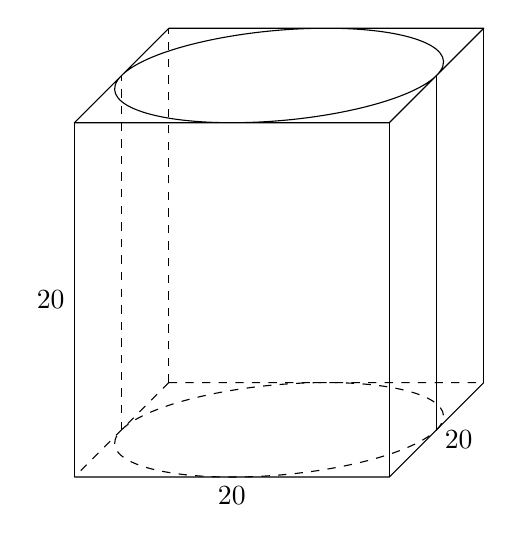
\begin{tikzpicture}[line join=round]
		\def\r{2} % bán kính đáy
		\def\h{4.5} % chiều cao
		% Đáy dưới
		\begin{scope}[yscale=.3,xslant=.3]
			\draw[dashed] (0,0) circle(\r);
			\draw
			(-\r,-\r) coordinate (A)
			--(\r,-\r) coordinate (B) node[below,midway]{20}
			--(\r,\r) coordinate (C) node[right=1mm,pos=.4]{20}
			(-\r,\r) coordinate (D)
			(-\r,0) coordinate (L)
			(\r,0) coordinate (R);
			\draw[dashed] (D)--(A) (D)--(C);
		\end{scope}
		% Đáy trên
		\begin{scope}[yshift=\h cm,yscale=.3,xslant=.3]
			\draw (0,0) circle(\r)
			(-\r,-\r) coordinate (At)
			--(\r,-\r) coordinate (Bt)
			--(\r,\r) coordinate (Ct)
			--(-\r,\r) coordinate (Dt)--cycle
			(-\r,0) coordinate (Lt)
			(\r,0) coordinate (Rt);
		\end{scope}
		\draw[dashed] (D)--(Dt) (L)--(Lt);
		\draw (A)--(At) node[left,midway]{20}
		(B)--(Bt) (C)--(Ct) (R)--(Rt);
	\end{tikzpicture}
\end{document}